%%T Illustration for reconstruction
%%D This is an illustration I made for my research related
%%D project. This uses .pic concept from tikz to reuse the
%%D same figure multiple times.
%%G research, tikz, pic
\usetikzlibrary{decorations.pathreplacing,}
\tikzset{
    photon/.style={fill,inner color=red,outer color=white,color=transparent!0},
    invisible/.style={color=transparent!0},
    cluster/.pic={ \tikzset{scale=5/10}
    \begin{scope}[yscale=-1]
        \draw[photon] (0.5,0.2) circle (8pt);
        \draw[photon] (-0.5,0.2) circle (8pt);
        \draw[photon] (0,0.6) circle (8pt);
        \draw[dashed] (-1.0,-0.1) -- (1.0,-0.1);
        \draw[photon] (-0.5,-0.5) circle (8pt);
        \draw[photon] (0.5,-0.5) circle (8pt);
        \draw (0,0) node[red,circle,minimum width=1.1cm] (#1) {};
    \end{scope}
    },
    avgcod/.pic={ \tikzset{scale=5/10}
    \begin{scope}[yscale=-1]
        \draw[dashed] (-1.0,-0.1) -- (1.0,-0.1);
        \draw[photon] (-0.5,-0.5) circle (8pt);
        \draw (0,0) node[red,circle,minimum width=13pt] (#1) {};
    \end{scope}
    }
}

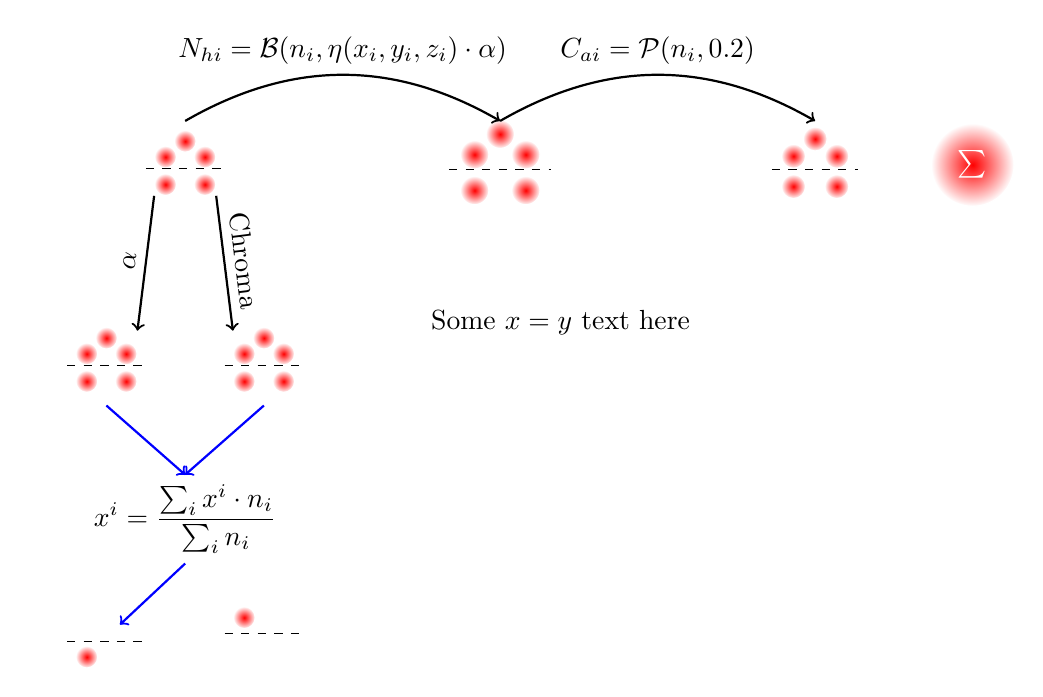
\begin{tikzpicture}[y=-1cm]
    \node[circle,minimum width=2cm] (B) at (0,0) {};
    \draw (1,0) pic {cluster=org};
    \draw (5,0)  pic[scale=1.3] {cluster=corner};
    \draw (9,0)  pic[scale=1.1] {cluster=ca};
    \draw (0,2.5) pic {cluster=alcca};
    \draw (2,2.5) pic {cluster=mccca};
    \draw (0,6) pic {avgcod=alca};
    \draw (2,6) pic[yscale=-1] {avgcod=mcca};
    \draw[photon] (11,0) circle (15pt) node {$\sum$};
    \draw[thick,->] (org.north)  to[out=30,in=150] node[above] {$N_{hi} = \mathcal{B}(n_i,\eta(x_i,y_i,z_i)\cdot \alpha)$} (corner.north);
    \draw[thick,->] (corner.north)  to[out=30,in=150] node[above] {$C_{ai} = \mathcal{P}(n_i,0.2)$} (ca.north);
    \draw[thick,->] (org.south west) -- node[sloped,above] {$\alpha$} (alcca.north east);
    \draw[thick,->] (org.south east) -- node[sloped,above] {Chroma} (mccca.north west);
    \node (wa) at (1,4.5) {$\displaystyle x^i = \frac{\sum_i x^i \cdot n_i}{\sum_i n_i}$};
    \node[right] (P) at (4,2) {Some $x=y$ text here };
    \draw[blue,thick,->] (wa.south) -- (alca);
    \draw[blue,thick,->] (alcca.south) -- (wa.north);
    \draw[blue,thick,->] (mccca.south) -- (wa.north);
\end{tikzpicture}

